\documentclass{article}

\usepackage[utf8]{inputenc}
\usepackage{enumitem}
\usepackage{float}
\usepackage{circuitikz}
\usepackage{todonotes}
\usepackage{amsmath}
\usepackage{tikz}
\usetikzlibrary{shapes, calc, shapes, arrows}
\usepackage{svg}


\title{Blatt 4}
\author{Luca Krüger, Jonas Otto, Jonas Merkle (Gruppe R)}
\date{\today}

\begin{document}
\maketitle

\section{Lernschritt im Perzeptron-Lernalgorithmus}

\begin{enumerate}[label=\arabic*.]
  \item $w^Tx+w_0 = 0 \iff y = -\frac{1}{2}x+\frac{1}{2}$
        \begin{figure}[H]
          \textit{}\centering
          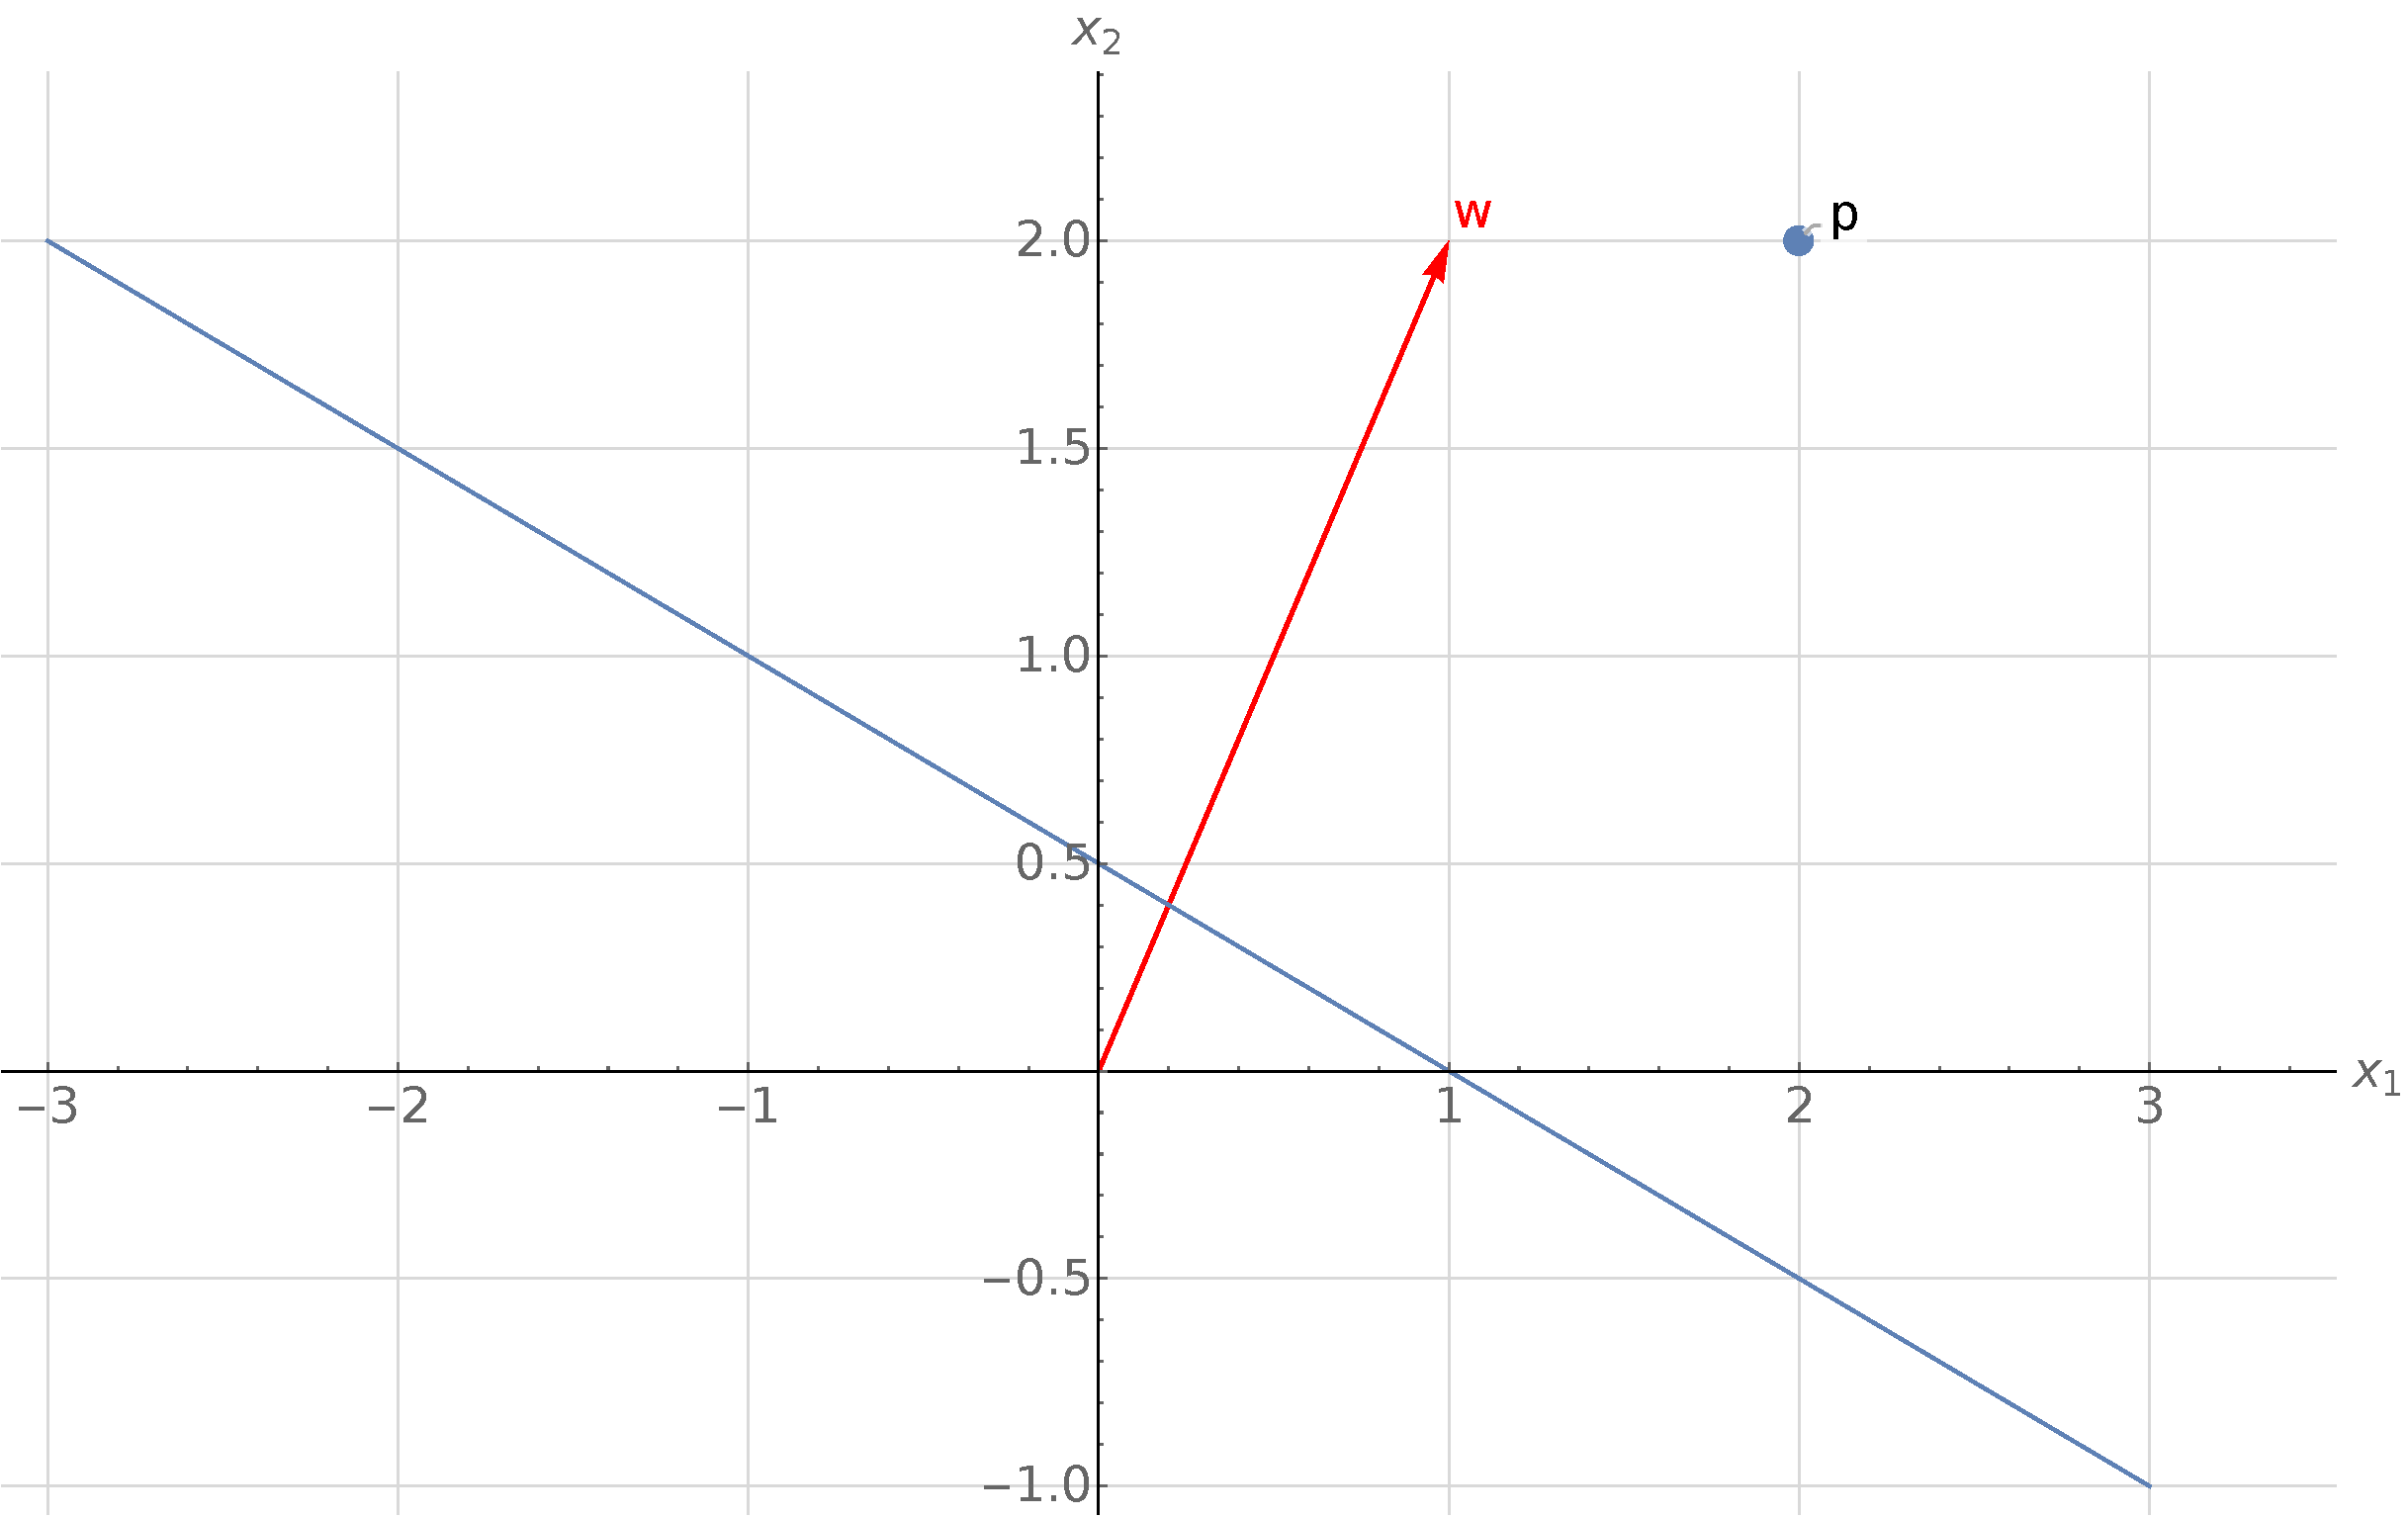
\includegraphics[width=\textwidth]{separation-line1.pdf}
          \caption{Separierungslinie}
        \end{figure}
  \item Bias in Gewichtsvektor $\mathbf{w}^*$:
        \begin{equation*}
          \mathbf{w}^* = \begin{pmatrix}
            1 \\ 2 \\ w_0
          \end{pmatrix}
        \end{equation*}

        \begin{equation*}
          \mathbf{p}^* = \begin{pmatrix}
            2 \\ 2 \\ 1
          \end{pmatrix}
        \end{equation*}

        % 3
  \item
        %$(\mathbf{w}^*)^T\mathbf{x}^* > 0$: Region auf Seite des Vektors $\mathbf{w}$ (Winkel zwischen $\mathbf{w}$ und $\mathbf{x} < 90^\circ$).
        \begin{figure}[H]
          \textit{}\centering
          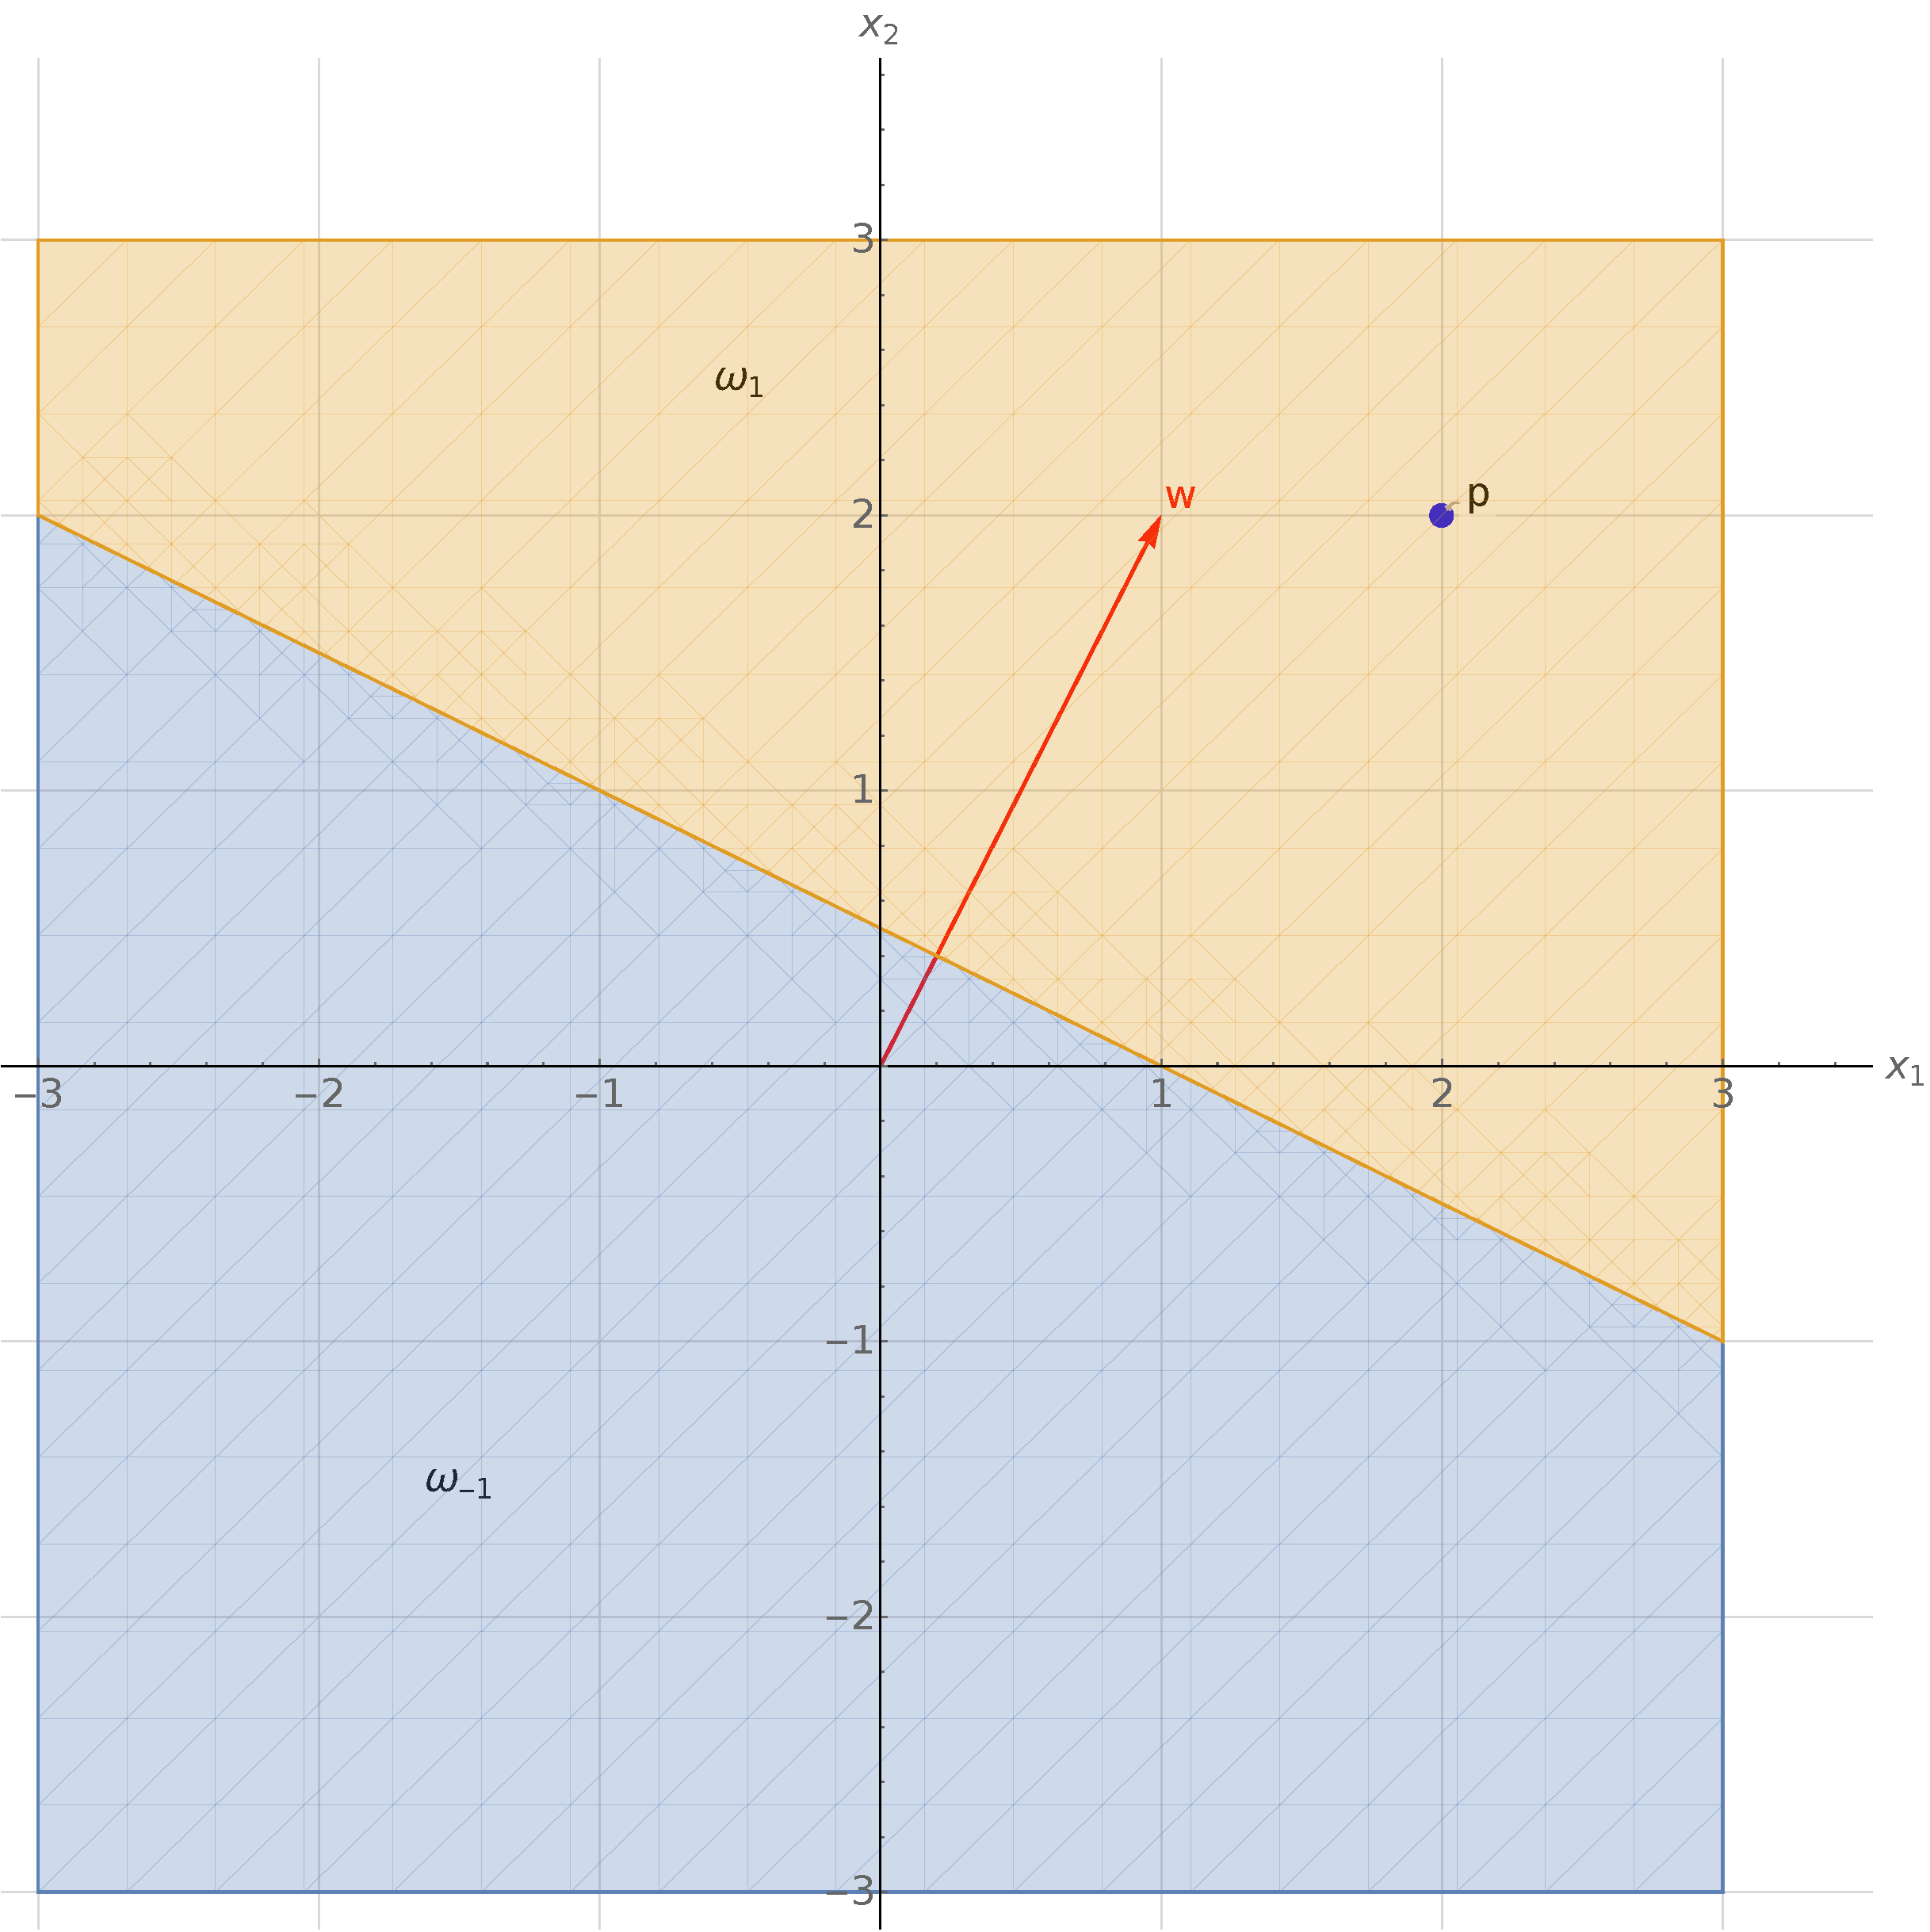
\includegraphics[width=\textwidth]{separation-regions1.pdf}
          \caption{Regionen}
        \end{figure}
        % 4
  \item Lernschritt I
        \begin{align*}
                        & w^*(t) \cdot p^* > 0 \ \ \wedge \ \ p^* \in \omega_{-1}                     \\ \\
          \Rightarrow   & w^*(t+1) = w^*(t) - p^* = \begin{pmatrix} -1 \\ 0 \\ -2 \end{pmatrix}                         \\
          \text{bzw.  } & \overset{\sim}{w}=\begin{pmatrix}-1 \\ 0\end{pmatrix}, \quad \overset{\sim}{w_0} = -2
        \end{align*}
  \item Visualisierung nach dem ersten Lernschritt
        \begin{figure}[H]
          \textit{}\centering
          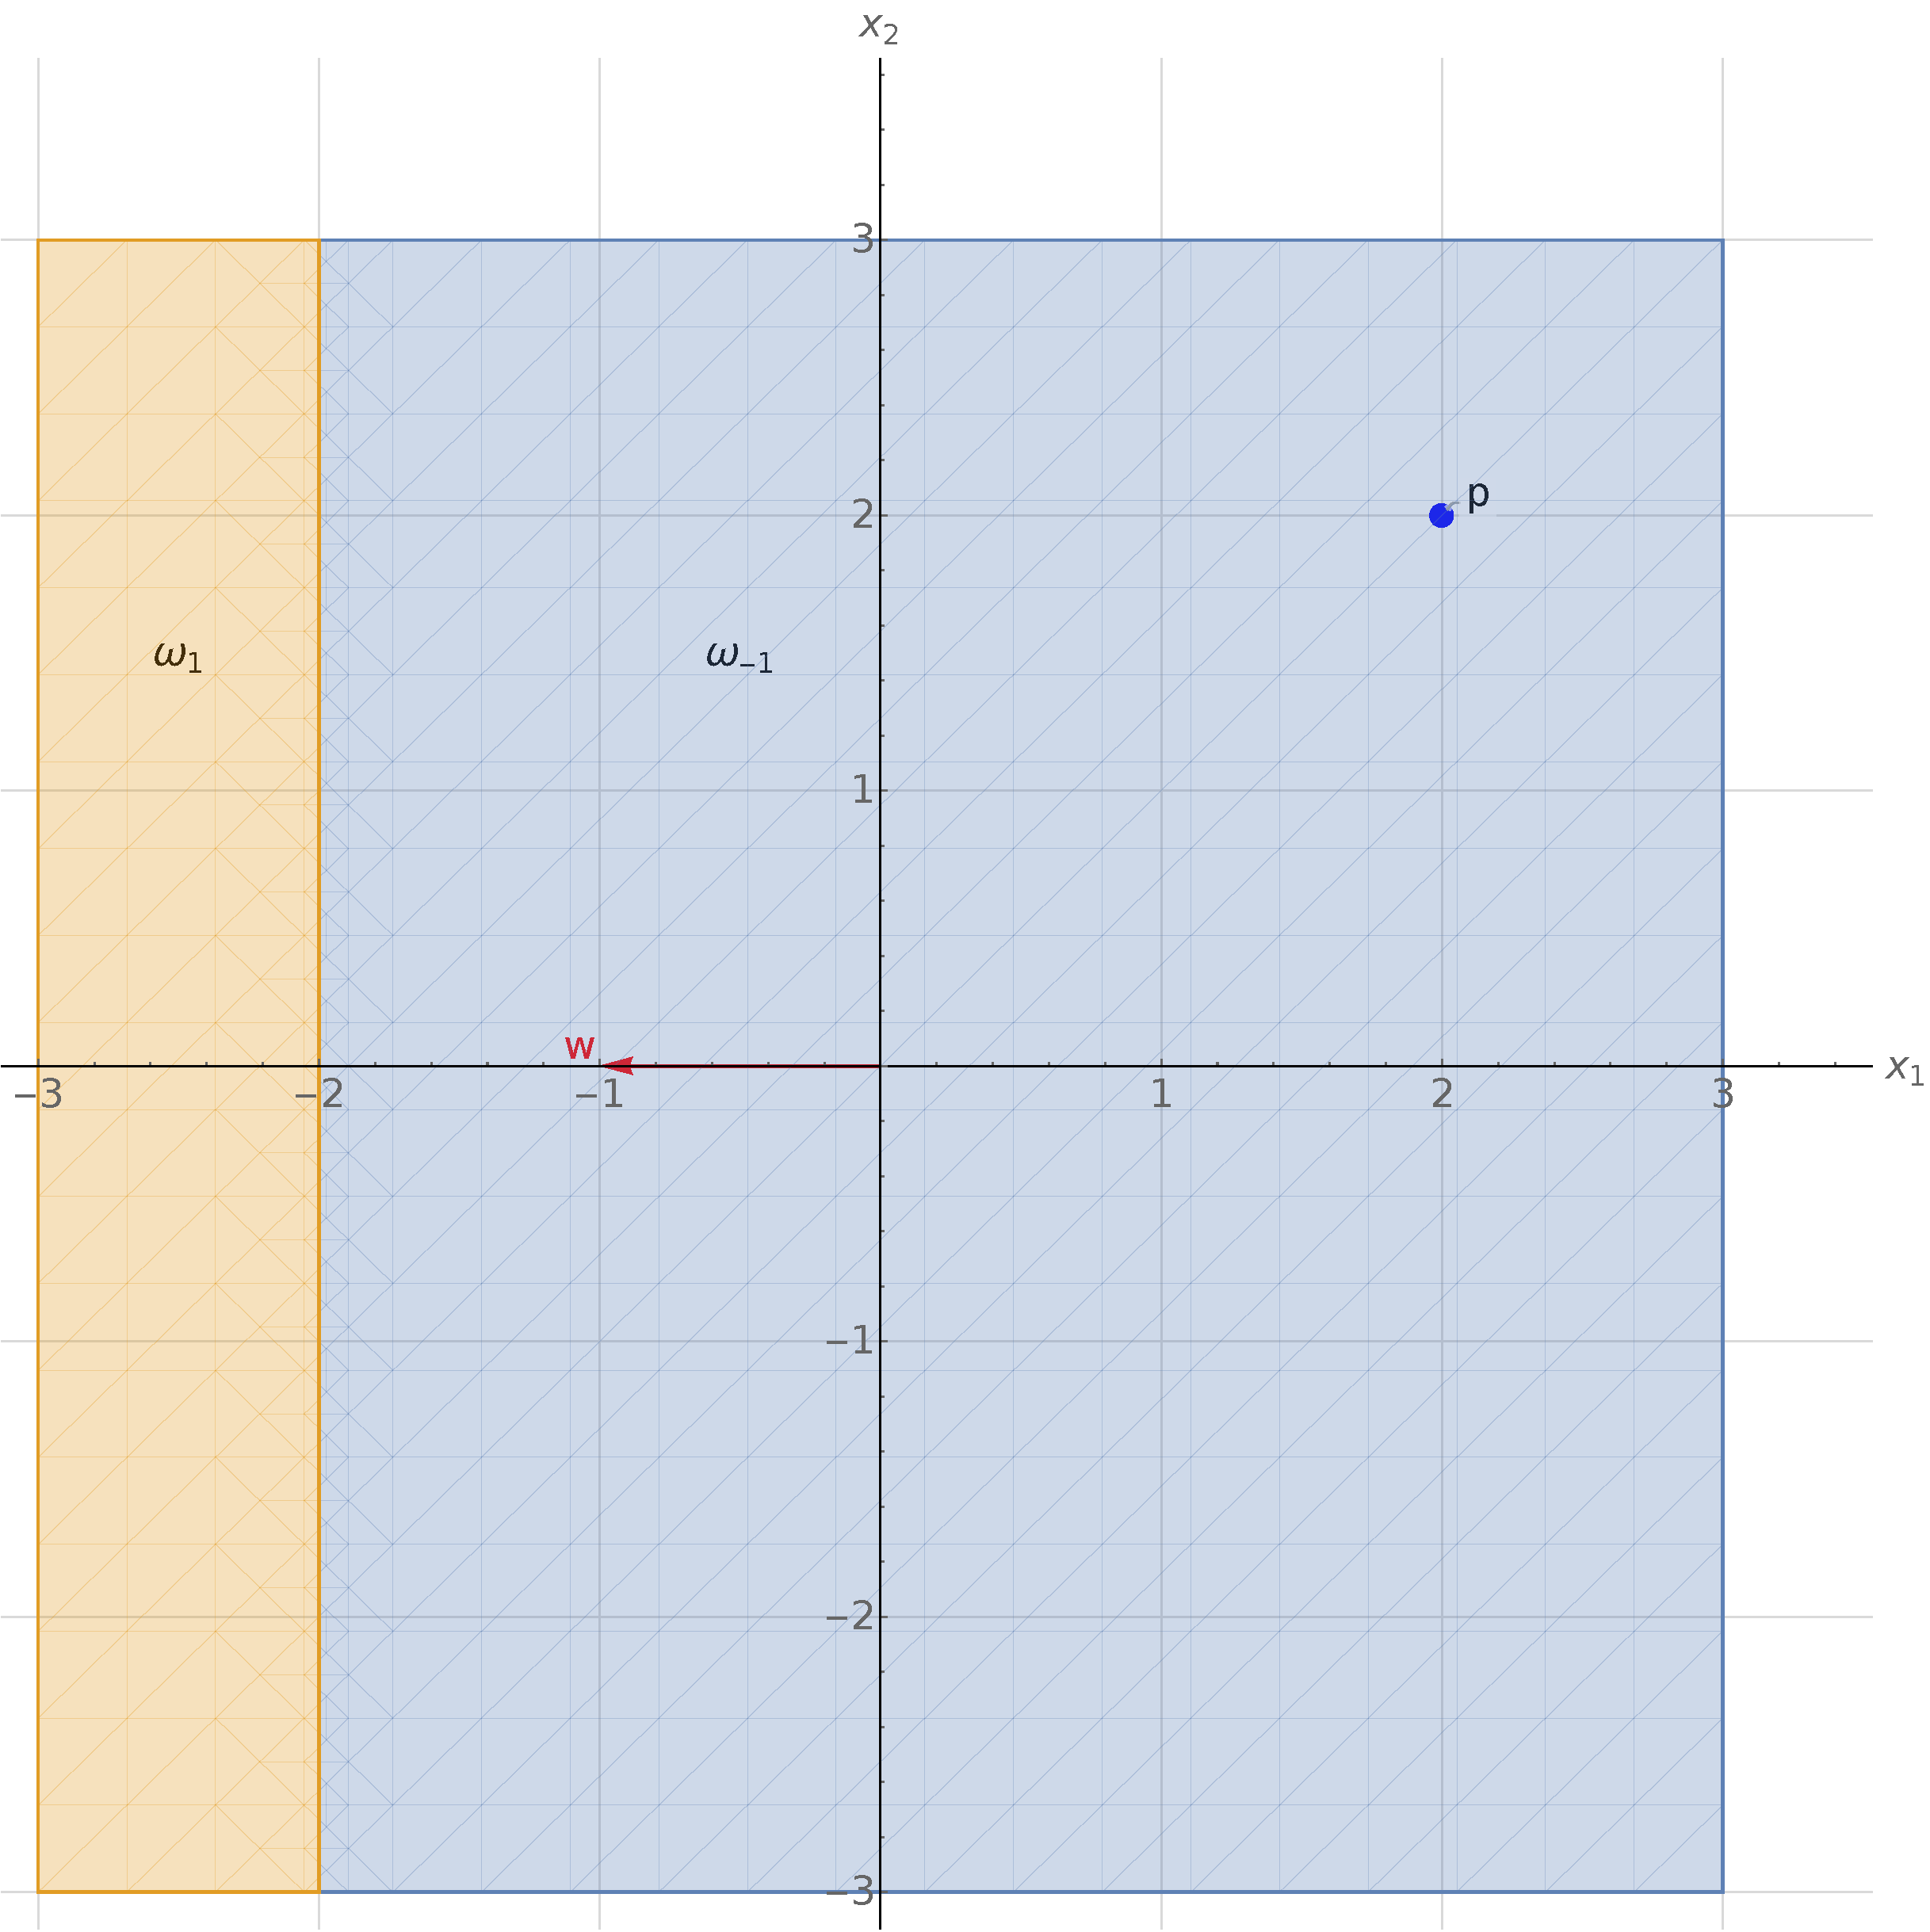
\includegraphics[width=\textwidth]{separation-regions2.pdf}
          \caption{Regionen nach dem ersten Lernschritt}
        \end{figure}
  \item Nach dem ersten Lernschritt liegt $p^*$ wie vom Lehrersignal vorgegeben in $\omega_{-1}$. Damit ist der Perzeptron-Lernalgorithmus abgeschlossen und weitere Iterationen führen zu keinen Änderungen von $\overset{\sim}{w}$
\end{enumerate}



\end{document}
